En esta sección se presentarán diversos artículos de investigación o tesis las cuales abordarán diversas técnicas y enfoques que se emplearon para afrontar problemas similares al de esta tesis. Asimismo, a continuación se presenta un cuadro resumen (véase Anexo \ref{A:table}) de lo que se presenta en esta sección.


\subsection{Real-time deep reinforcement learning based vehicle navigation \citep*{pr_koh}}
\citeauthor{pr_koh} realizaron un artículo de investigación el cual fue publicado en la revista «Applied Soft Computing» en el año 2020. Este fue titulado \citetitle{pr_koh} la cual traducida al español significa «Navegación de vehículos basada en aprendizaje de refuerzo profundo en tiempo real».

\subsubsection{Planteamiento del Problema y objetivo }
Los autores del siguiente artículo mencionan la gravedad del problema de la congestión vehícular en las ciudades contemporáneas, teniendo como consecuencia el alto consumo innecesario de energía, la contaminación y el tiempo invertido en viaje. Además, menciona la dificultad que tienen los algoritmos existentes para la optimización de las carreteras con el fin de afrontar dicho problema, siendo esta la complejidad que tienen los vehículos al interactuar en un entorno dinámico en tiempo real. Por lo que el objetivo de los autores es implementar un modelo de aprendizaje por refuerzo profundo (DRL) con el fin de construir un sistema de navegación en tiempo real a través de una secuencia de decisiones.

\subsubsection{Metodología empleada por los autores}
Este artículo propone un framework el cual primero construye una simulación en SUMO, que contiene una interfaz de Control de Tráfico (TraCI) y que utiliza mapas urbanos reales en OpenStreetMap mediante el método NETCONVERT. Luego en la misma simulación de SUMO, se puede extraer y pre procesar los datos a través del método TraCI que recupera el número de vehículos, el tiempo de viaje esperado, y la posición actual y el destino.

La segunda parte del framework propuesto es el middleware, que conecta el entorno de SUMO con las redes neuronales DRL bajo un método mejorado de Deep Q-Learning Network (DQN) para mantener y actualizar las políticas de navegación y proporciona comandos para la navegación. El modelo propuesto contiene un esquema de exploración de dos etapas que buscan mejorar la convergencia de la red así como su velocidad. La primera etapa se utiliza la política convencional y la segunda etapa es un método basado en la distancia para reemplazar la selección de una ruta. La estructura de la red neuronal profunda contiene 5 capas conectadas, la primera capa de entrada contiene 150 neuronas, las dos capas ocultas tienen 100 neuronas bajo la función de activación RELU, una estructura de duelo y su capa de salida. %\medskip

\begin{figure}[h]
	\begin{center}
		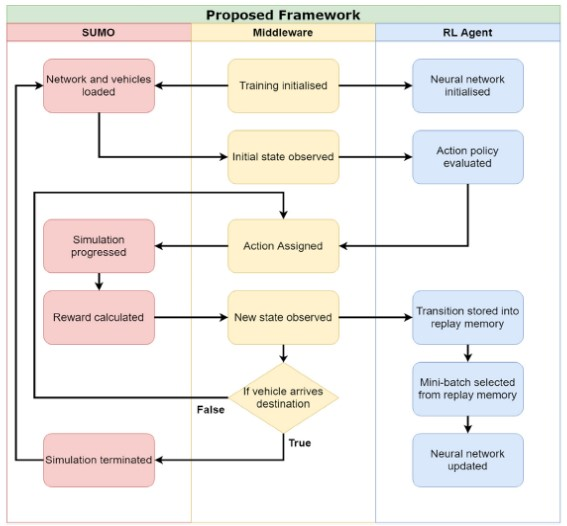
\includegraphics[width=0.65\textwidth]{2/figures/SUMO.jpg}
		\caption{Framework propuesto}
		\label{1:fig2}
	\end{center}
\end{figure}
%%%Ecuacion
%\begin{equation}  
%\label{eq:RMSE}
%RMSE = \sqrt{\frac{\sum_{i=1}^{N}{\Big(O_i -T_i\Big)^2}}{N}}
%\end{equation}

\subsubsection{Resultados obtenidos}
Para demostrar la eficiencia del modelo propuesto, se compara con diferentes modelos por ciudad, los resultados de una ciudad demuestran que el modelo reduce como máximo el tiempo de viaje en 5.3\%, 5.1\% y 16.4\% dependiendo de la demanda del tráfico. Otro indicador que se utiliza para medir su eficacia es la prueba de Wilcoxon, demostrando que el modelo propuesto es superior a los demás modelos.%\medskip

\begin{figure}[h]
	\begin{center}
		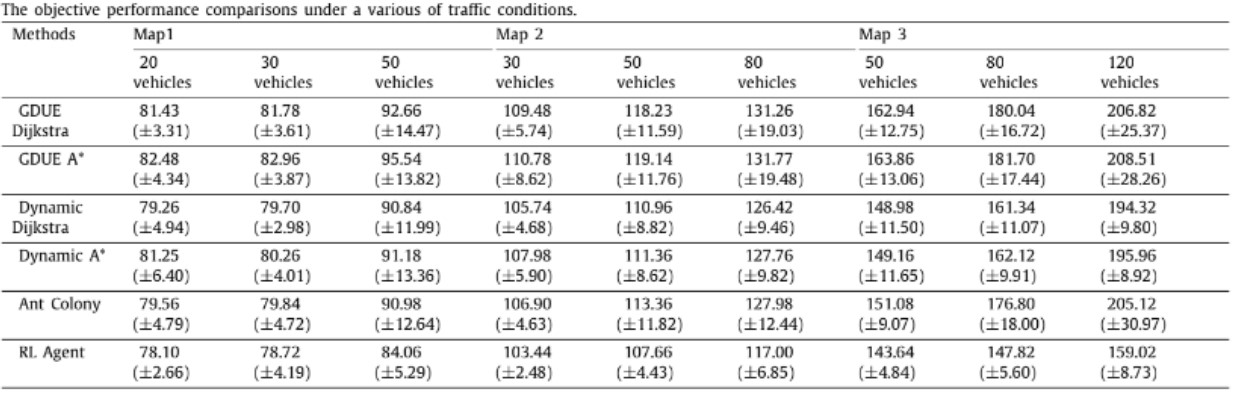
\includegraphics[width=0.65\textwidth]{2/figures/ResultSumo.jpg}
		\caption{Comparación de rendimiento de los modelos}
		\label{1:fig2}
	\end{center}
\end{figure}

%\medskip

 \begin{figure}[h]
	\begin{center}
		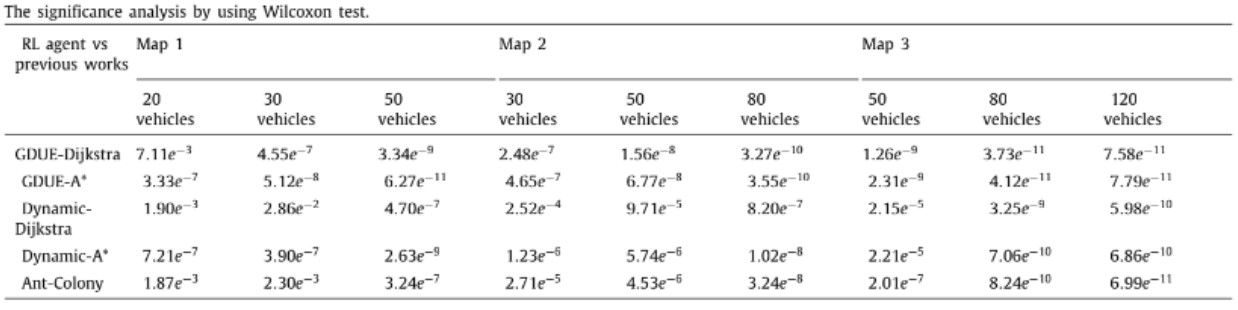
\includegraphics[width=0.65\textwidth]{2/figures/Result2Sumo.jpg}
		\caption{Análisis de significancia de los modelas con la prueba de Wilcoxon}
		\label{1:fig2}
	\end{center}
\end{figure}

\subsection{SafeRoute: Learning to navigate streets safely in an urban environment \citep*{pr_saferoute}}
\citeauthor{pr_saferoute} realizaron un artículo de investigación el cual fue publicado en la revista «ACM Transactions on Intelligent Systems and Technology» en el año 2020. Este fue titulado \citetitle{pr_saferoute} la cual traducida al español significa «SafeRoute: aprender a navegar por las calles de forma segura en un entorno urbano».

\subsubsection{Planteamiento del Problema y objetivo }
Ante los resultados de estudios realizados en la Universidad de Cornell y Hollaback en 2014, se muestra que el 85\% de mujeres tomaron rutas diferentes para ir a su destino con el fin de evitar ser víctimas de acoso o agresión. También se menciona la necesidad de las personas, como los turistas, de contar con una aplicación que pueda detectar rutas seguras. Con esto en mente, se propone SafeRoute, que es una solución de estos problemas utilizando algoritmos de aprendizaje por refuerzo profundo, que tiene ventaja bajo los algoritmos clásicos como Dijkstra, ya que es una opción a problemas que requieren tomar decisiones incrementales por cada intersección que se presenta entre el origen y el destino, además que tiene la ventaja de adaptarse a nuevos datos sin requerir a ser entrenado nuevamente.


\subsubsection{Metodología empleada por los autores}
Se emplea información pública de delitos de la ciudad de Nueva York, San Francisco y Boston, y se filtra los tipos de delitos relacionados con acoso callejero y asalto, los cuales son tiroteo, asalto y robo. Asimismo, para la obtención cartográfica de dichas ciudades, se utilizó OpenStreetMap (OSM).
%\medskip

\begin{figure}[h]
	\begin{center}
		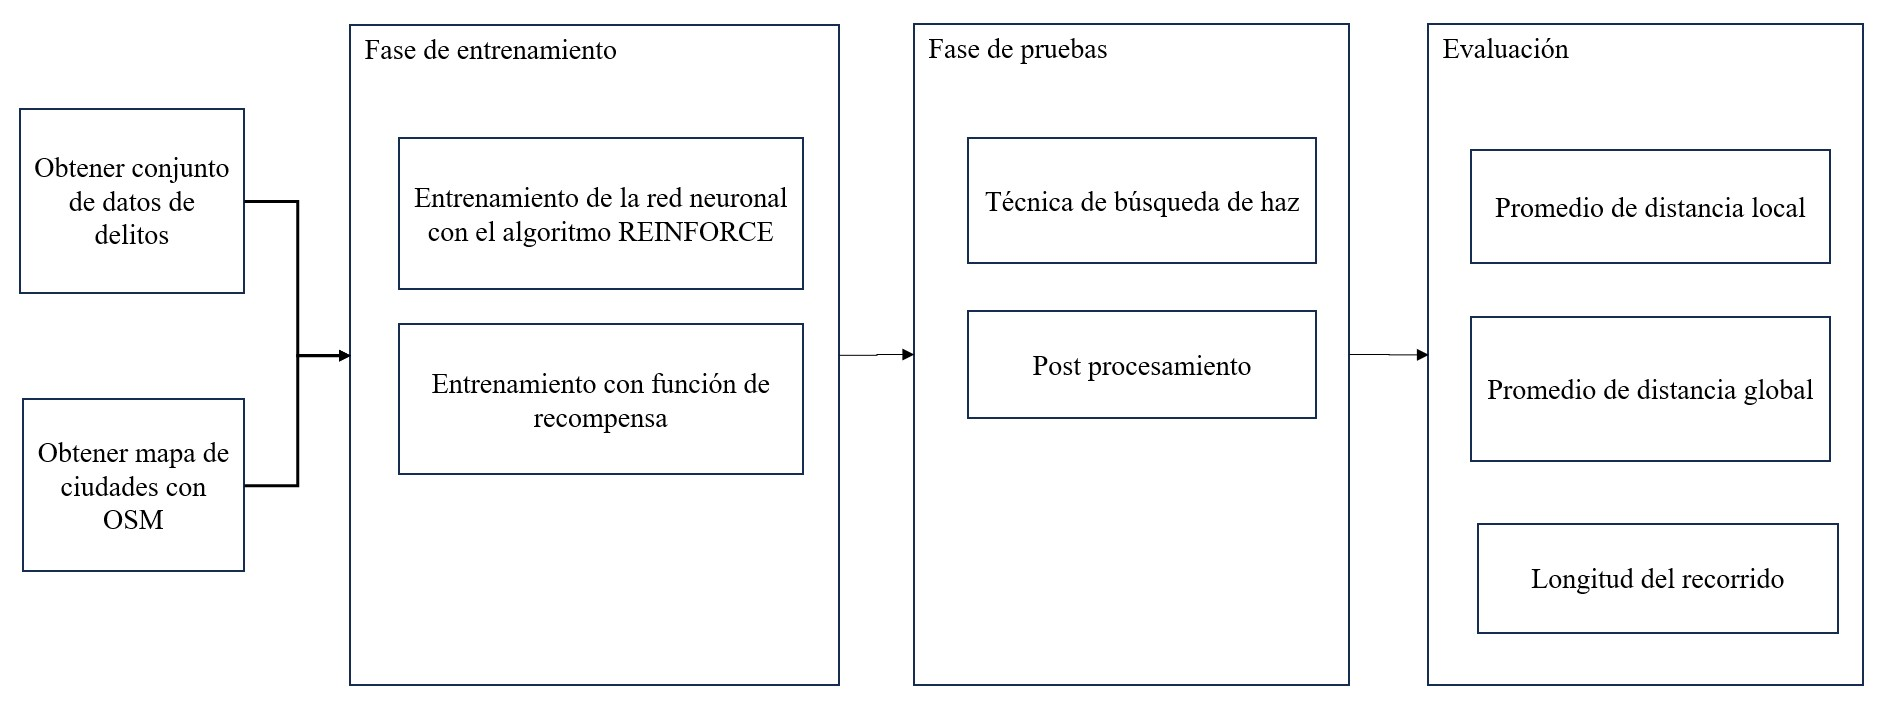
\includegraphics[width=0.65\textwidth]{2/figures/SafeMetodo.jpg}
		\caption{Metodología propuesta por los autores}
		\label{1:fig2}
	\end{center}
\end{figure}

De acuerdo a la metodología propuesta por los autores, la arquitectura se divide en dos partes, la primera es donde interviene la red neuronal de aprendizaje por refuerzo, y el segundo es la red de políticas definidas para que la red neuronal utiliza al momento de tomar decisiones. Este entorno se presenta como proceso de decisión de Markov con tuplas que contienen los estados contínuos del mapa, las acciones disponibles para el algoritmo y la probabilidad de pasar de un estado a otro.
%\medskip

\begin{figure}[h]
	\begin{center}
		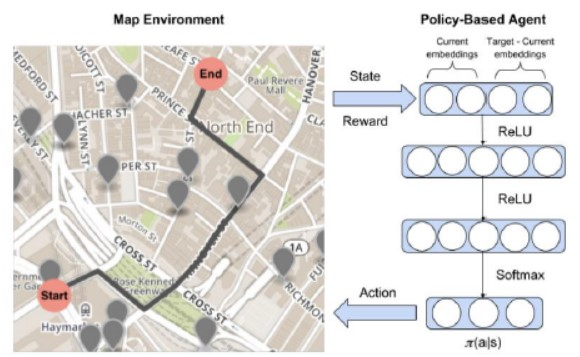
\includegraphics[width=0.65\textwidth]{2/figures/safeRouteAgent.jpg}
		\caption{Estructura de la red neuronal del modelo propuesto}
		\label{1:fig2}
	\end{center}
\end{figure}

Se establece una función de recompensa para optimizar las múltiples preferencias del modelo, en este caso es evitar las áreas de crimen al crear una ruta. La definición de esta función se establece de la siguiente manera:
%\medskip
\begin{figure}[h]
	\begin{center}
		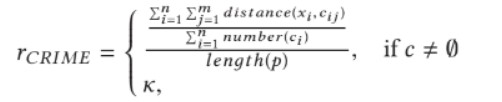
\includegraphics[width=0.65\textwidth]{2/figures/EcuacSafe.jpg}
	\end{center}
\end{figure}

Donde n es el número de bordes de cada camino, m es el número de delitos de cada nodo, x es la lista de puntos de cada camino, c es la lista de delitos de cada radio, p es el recorrido y k es un hiper parámetro.

En la fase de entrenamiento, consta de dos partes, la primera es el pre entrenamiento de la red neuronal para detectar rutas más cortas, en este proceso se utilizan técnicas de aprendizaje por refuerzo, específicamente el algoritmo Monte Carlo Policy Gradient (REINFORCE) para que actualice los parámetros de la red neuronal. La segunda es el entrenamiento con recompensas, donde se entrena nuevamente a la red neuronal considerando la seguridad en cada ruta, premiandolo por evitar áreas con alto índice de crimen, el cuál es la función de recompensa, y de esta manera actualizando la política de la red neuronal.

En la fase de pruebas, se utiliza una técnica de búsqueda de haz para encontrar varias rutas potenciales, luego se realiza un post procesamiento que evite bucles externos que se hayan creado durante la navegación, con el fin de que la ruta generada sea coherente y eficiente.
Para la evaluación del modelo propuesto con respecto a otros modelos, se aplicaron métricas cómo el promedio de la distancia local, el promedio de la distancia global y la longitud del recorrido. 

\subsubsection{Resultados obtenidos}
El modelo propuesto se comparó con el algoritmo de Dijkstra y SafePath, el cual crea produce caminos no dominados tomando en cuanto la seguridad. Se obtuvieron los mejores resultados con una tasa de aprendizaje de 0.0005 y realizando 5 saltos para un primer entrenamiento y luego 10 saltos. %\medskip

\begin{figure}[h]
	\begin{center}
		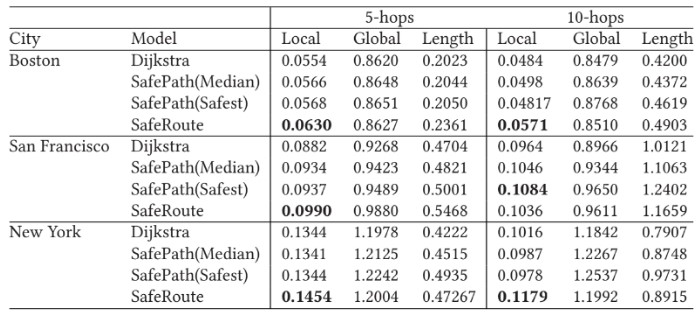
\includegraphics[width=0.65\textwidth]{2/figures/resultSafe.jpg}
		\caption{Comparación de rendimiento de los modelos}
		\label{1:fig2}
	\end{center}
\end{figure}

Se observa que las distancias entre un ruta a la zona de crimen, el que presenta un valor más bajo es Boston, debido a su densidad de criminalidad, mientras que las rutas generadas en Nueva York son las que más se alejan. Sin embargo, se demuestra que tanto en la época 5 como la época 10, el modelo propuesto SafeRoute supera al modelo Dijkstra y los modelos de SafePath, a excepción de la ciudad de San Francisco, el cuál el número que más se aleja de los riesgos es el modelo más seguro de SafePath en la época 10.

\subsection{Predicting motor vehicle theft in Santiago de Chile using graph-convolutional LSTM \citep*{pr_esquivel}}
\citeauthor{pr_esquivel} realizaron un artículo de investigación el cual fue presentado en la «39th International Conference of the Chilean Computer Science Society» en el año 2020. Este fue titulado \citetitle{pr_esquivel} la cual traducida al español significa «Predicción del robo de vehículos de motor en Santiago de Chile utilizando LSTM gráfico convolucional».

\subsubsection{Planteamiento del Problema y objetivo }
Ante el problema del incremento de autos robados en Chile en el año 2017, se menciona que este tipo de delitos, que, si bien es de bajo riesgo, puede desencadenar otros delitos más graves como el contrabando de armas o drogas, o crímenes internacionales. Es por esto que a través de un modelo de predicción de robo de vehículos puede contribuir a la mitigación y mayor seguridad por parte de la fuerza policial en las zonas con mayor probabilidad de robos. En este trabajo de investigación busca crear una nueva metodología para la predicción de robos de vehículos en la ciudad de Santiago de Chile desarrollando una red neuronal convolucional LSTM basada en grafos (GCLSTM) utilizando la técnica de preprocesamiento de datos, la cuál es la regresión LOESS.


\subsubsection{Metodología empleada por los autores}
Los autores proponen la siguiente metodología: %\medskip


\begin{figure}[h]
	\begin{center}
		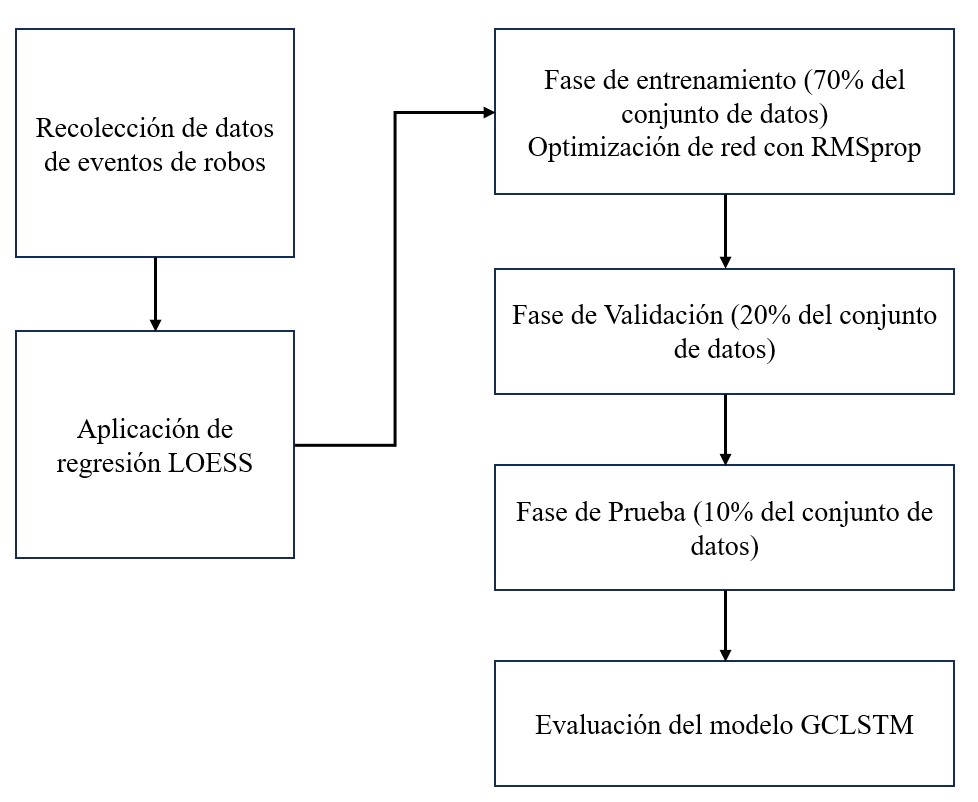
\includegraphics[width=0.65\textwidth]{2/figures/ChileMetodo.jpg}
		\caption{Metodología propuesta por los autores}
		\label{1:fig2}
	\end{center}
\end{figure}

El primer paso de esta metodología empieza con la recolección de los datos, que en este caso son los eventos de robos de vehículos en las comunas de la Región de Chile del año 2015 al 2019, que contiene un total de 129.127 registros. Luego se procedió a realizar la suma de los eventos de robo por día de cada comuna para la creación de una serie de tiempo y posterior a esto, aplicar la regresión LOESS, el cual es una técnica no paramétrica que utiliza los mínimos cuadrados ponderados para asignar un mayor peso a los más cercanos y menos a los que están más lejos. La aplicación de dicha técnica permite la reducción de ruido de la serie de tiempo. De este paso, se obtuvo una matriz suavizada de número de eventos de robos, el cuál sirve como input para la red GCLSTM. 

Dicha red suma las matrices de adyacencia e identidad para realizar la convolución con parámetros K, luego se le asigna a cada vecino un peso por iteración y estas van a las compuertas LSTM para la extracción de la última celda para el desarrollo de una capa de salida lineal con la función tanh. Para la optimización de la red GCLSTM, se aplicó el algoritmo de RMSprop para entrenar el modelo hasta que haya un sobreajuste en los datos.

%\medskip

\begin{figure}[h]
	\begin{center}
		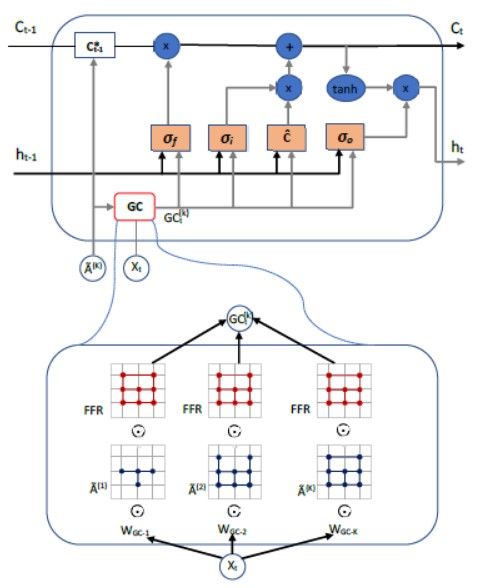
\includegraphics[width=0.65\textwidth]{2/figures/EsquivelRed.jpg}
		\caption{Estructura de la red convolucional LSTM basada en grafos}
		\label{1:fig2}
	\end{center}
\end{figure}

Para la fase de entrenamiento, se utilizó el 70\% del conjunto de datos, 20\% de validación y 10\% para la fase de prueba.

\subsubsection{Resultados obtenidos}
Como parte de los resultados, en la fase de entrenamiento, se entrenó en el modelo tradicional LSTM y el modelo GCLSTM, dando como resultado que a partir de la iteración 31, la curva MSE del modelo GCLSTM desciende más que el tradicional. 
Mientras que, en la fase de pruebas, se demuestra, con la métrica R2, que el modelo propuesto obtuvo 0.86, y el modelo LSTM tuvo 0.70, teniendo una mayor similitud la red GCLSTM entre lo esperado con lo observado. Por otra parte, el MSE del modelo propuesto fue 0.014 y el modelo LSTM es de 0.031; demostrando que el modelo puede obtener patrones temporales y espaciales para la predicción de crimen en distintas zonas de una ciudad. 

\subsection{Algoritmo para calcular la ruta más segura y óptima \citep*{pr_areiza}}
\citeauthor{pr_areiza} realizaron un artículo de investigación el cual fue publicado en el año 2022. Este fue titulado \citetitle{pr_areiza}.

\subsubsection{Planteamiento del Problema y objetivo }
La creciente cifra de casos de acoso callejero en las calles de Medellín, así como casos de asaltos y violación, ha tenido como consecuencia que el miedo de las mujeres aumente y por ende, se sientan inseguras por cuál ruta tomar. A pesar de los distintos métodos de prevención, se menciona que no siempre son efectivos para evitar ser víctima de acoso en espacios públicos. Además, aplicaciones de generación de rutas para el transporte, como Google Maps o Waze, no cuentan con la capacidad de detectar rutas seguras, ya que es propio sistema de estas sólo calculan sus rutas en base a la distancia más corta. Este trabajo de investigación busca solucionar este problema implementando el algoritmo de Dijkstra, para calcular tres caminos diferentes tomando en cuenta la distancia y el índice de riesgo.

\subsubsection{Metodología empleada por los autores}
Para la obtención del mapa de Medellín, se empleó Open Street Maps (OSM) en Python, el cual contiene en cada segmento su longitud en metros, en qué sentidos va, y sus representaciones binarias proporcionadas por la propia librería OSM. Para el cálculo del riesgo, se empleó un conjunto de datos de la encuesta de calidad de vida de Medellín del año 2017; luego se procedió a realizar una combinación lineal (CL)  mediante el análisis de componentes principales, el cual  es la máxima varianza de la proporción de hogares que se sienten inseguros entre la proporción de hogares que tienen ingresos inferiores al salario mínimo; después se normaliza la combinación lineal y la proporción de esta es considera como el riesgo de acoso.
%\medskip

\begin{figure}[h]
	\begin{center}
		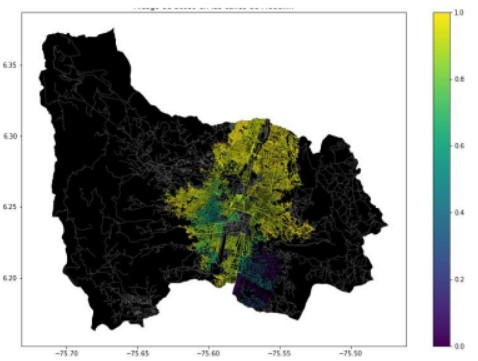
\includegraphics[width=0.65\textwidth]{2/figures/segmento.jpg}
		\caption{Riesgo de acoso sexual mediante combinación lineal}
		\label{1:fig2}
	\end{center}
\end{figure}

Se crea un diccionario que almacena el peso de cada vértice mediante el producto entre la longitud y riesgo de acoso de cada relación entre origen y destino. Se implementa el algoritmo de Dijkstra que requiere de tres parámetros los cuáles son los grafos creados, y los vértices de origen y destino. Este algoritmo calcula cada vecino del vértice actual a través de sus pesos que están almacenados en el diccionario para calcular el camino con menos peso. Además del cálculo tradicional que emplea, el cuál es r*d, donde r es el riesgo de acoso, y d es la distancia en metros, se calculó dos caminos más. El primero es la suma entre la distancia y el riesgo, mientras que el segundo eleva la distancia al riesgo de acoso. Para graficar estos tres resultados, se empleó la librería GmPlot, une el camino del origen y destino mediante las coordenadas ubicadas en Google maps, siendo más fácil de visualizar para el usuario.
%\medskip


\begin{figure}[h]
	\begin{center}
		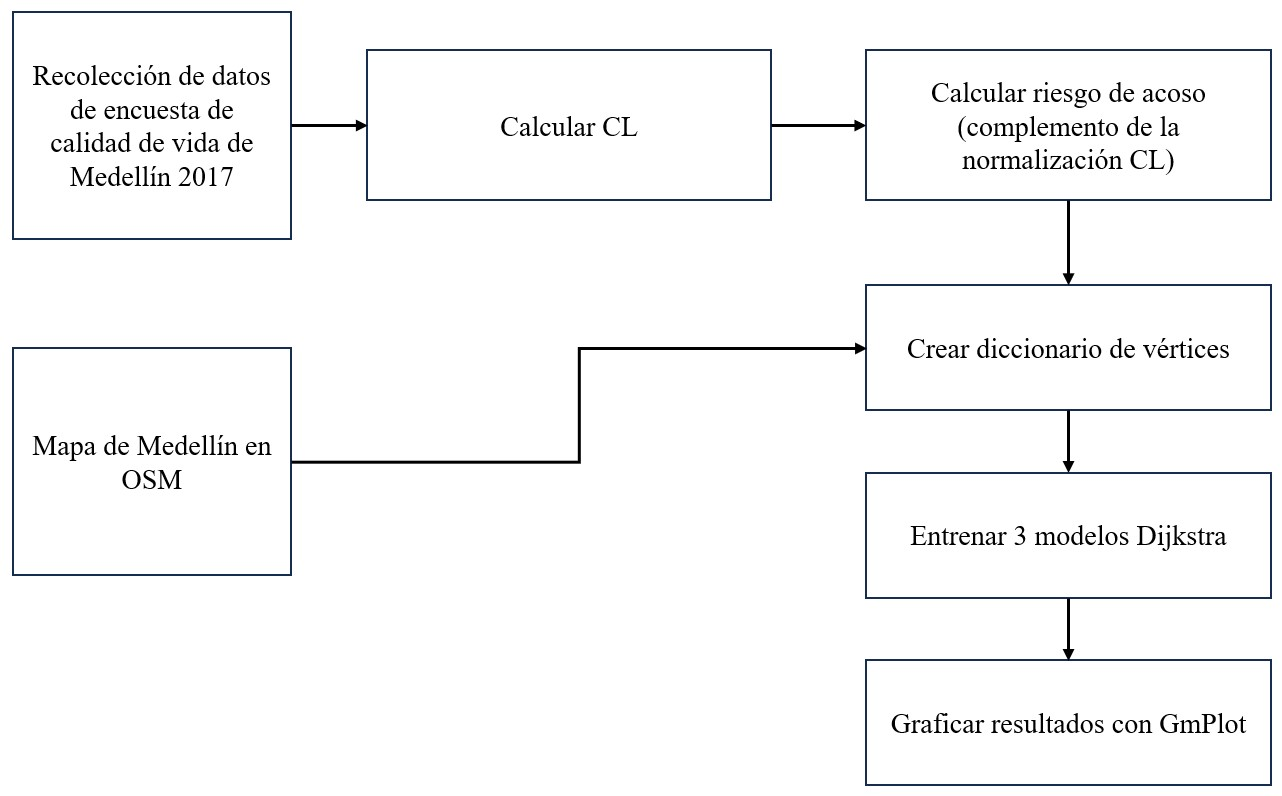
\includegraphics[width=0.65\textwidth]{2/figures/medellinMetodo.jpg}
		\caption{Metodología propuesta por los autores}
		\label{1:fig2}
	\end{center}
\end{figure}

\subsubsection{Resultados obtenidos}
Se presenta los resultados que son obtenidos por el algoritmo, estableciendo el origen en la Universidad EAFIT hasta la Universidad Nacional, el cual se puede visualizar en la siguiente tabla:%\medskip

\begin{table}[h]
	\centering
	\begin{tabular}{c|c|c|c}
		Camino & Distancia & Riesgo & Tiempo de ejecución\\\hline
		r*d & 9061.75m & 0.58& 1.01033s\\
		r+d & 8574m& 0.69& 1.01030s\\
		d\^r& 16642m& 0.35& 1.00640s
	\end{tabular}
	\caption{\label{tab:results}Tabla de resultados.}
\end{table}

%\medskip

Se observa que en términos de evitar el mayor riesgo, la mejor opción es el tercer camino (d\^r); sin embargo, la distancia que puede recorrer una persona es amplia a comparación de los otros caminos; asimismo, la opción más balanceada en cuanto al índice de riesgo y la distancia recorrida es el primer camino (r*d). También se demuestra que el tiempo de ejecución es bastante bajo, por lo que abre la oportunidad de ser empleado en una aplicación móvil para el fácil uso de los usuario que lo emplearán en su vida cotidiana.


%%%%%%%%%%%%%%%%%%%%%%%%%%%%%%%%%%%%%%%%%%%%%%%%%%%%%%%%%%
\subsection{Route-the safe: A robust model for safest route prediction using crime and accidental data \citep*{pr_Soni}}
\citeauthor{pr_Soni} realizaron un artículo de investigación el cual fue publicado la entrevista en el año 2019. Este fue titulado \citetitle{pr_Soni} la cual traducida al español significa «Ruta segura: un modelo sólido para la predicción de rutas más seguras utilizando datos sobre delitos y accidentes».

\subsubsection{Planteamiento del Problema y objetivo }
La falta de conocimiento de la zona de una ciudad para un turista, así como invertir su tiempo en investigar sobre esta, puede crear una dependencia a sus conductores o pueden verse expuestas a ciertos peligros, como el robo de sus pertenencias. Asimismo, también se menciona la falta de capacidad que tienen las aplicaciones de rutas al momento de elegir un camino seguro. Con el objetivo de ser una herramienta de ayuda a la hora de elegir la ruta más segura para viajar, este proyecto  utiliza algoritmos de aprendizaje automático para la predicción de rutas seguras mediante el cálculo de puntuación de riesgo de cada ruta de las ciudad de Nueva York utilizando datos sobre delitos y accidentes.
\subsubsection{Metodología empleada por los autores}
Este trabajo de investigación presenta la siguiente metodología utilizada para la implementación de su modelo:
%\medskip

\begin{figure}[h]
	\begin{center}
		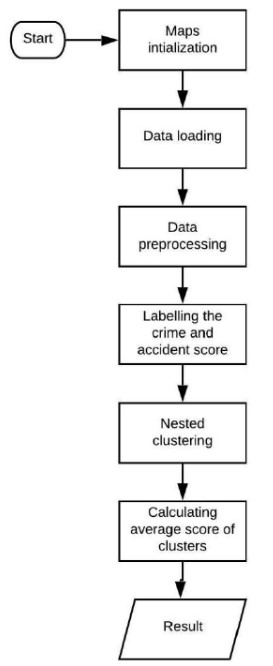
\includegraphics[width=0.35\textwidth]{2/figures/routeMet.jpg}
		\caption{Metodología Propuesta}
		\label{1:fig2}
	\end{center}
\end{figure}
%\medskip
Como primer paso de la metodología propuesta, se inicializa el mapa con el API de Google Maps, para luego proceder a configurar su función gmaps. Luego se cargan los datos, los cuáles contienen datos de delitos y accidentes desde el sitio web de datos abiertos de Nueva York, que brindan información del tipo de delito o accidente, así como su latitud y longitud. El siguiente paso se aplica al preprocesamiento de los datos para limpiar los datos atípicos o faltantes.
Una vez realizado el preprocesamiento de los datos, se procede a etiquetar la puntuación de accidentes de un punto (AS) y la puntuación de delitos de un punto (CS). Para la puntuación de delitos se asigna ponderaciones que van desde 1 a 15 dependiendo del delito y tipo de castigo que se le impone al sospechoso. Mientras que la puntuación de accidentes se calcula de la siguiente manera:

AS = PK*2 + CK*2 + MK*2 + PI + CI + MI

	Donde:

PK: Recuento de peatones fallecidos

CK: Recuento de ciclistas fallecidos

MK: Recuento de automovilistas fallecidos

PI: Recuento de peatones heridos

CI: Recuento de ciclistas heridos

MI: Recuento de automovilistas heridos

El siguiente paso es la formación de los grupos utilizando K Means, que es un algoritmo de agrupación de aprendizaje automático no supervisado, basado en la latitud y longitud, así como los conjuntos de datos se concatenan para agruparlos y determinar las regiones de riesgo. Específicamente, primero se agrupa en función a la longitud y latitud donde ocurrieron los hechos, para dividir el mapa de Nueva York en regiones más pequeñas. Asimismo, para generar las regiones de riesgo, se agrupa bajo los grupos ya formados en un distrito, como por ejemplo, el distrito de Manhattan. 

Después de hacer las agrupaciones de los grupos formados de un distrito, se realiza la puntuación promedio de cada agrupación, los cuáles se calculan de la siguiente manera:
%\medskip
\begin{figure}[h]
	\begin{center}
		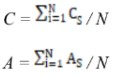
\includegraphics[width=0.25\textwidth]{2/figures/agrupSafe.jpg}
	\end{center}
\end{figure}
%\medskip
Donde N es el número de puntos de un grupo. Después se procede a calcular la puntuación del riesgo (RS) que toma como entrada el origen y destino de la ruta a calcular gracias al API de google maps llamado Direction Service,  que proporciona una serie de pasos al usuario para seguir la ruta. Luego se utiliza el modelo KNN Regresor para hallar el vecino más cercano según el grado de riesgo de cada punto. La puntuación de riesgo (RS) se calcula de la siguiente manera: 

%\medskip
\begin{figure}[h]
	\begin{center}
		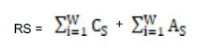
\includegraphics[width=0.25\textwidth]{2/figures/riesgoSafe.jpg}
	\end{center}
\end{figure}
%\medskip

Donde W es el número de puntos de rutas que hay entre el origen y el destino.

Como último punto, el modelo debe mostrar la ruta más segura bajo las siguientes dos condiciones: el primero es que la ruta debe presentar la puntuación de riesgo más baja, y la segunda es que si hay más de una ruta segura, se debe elegir la distancia más corta.
%\medskip
\begin{figure}[h]
	\begin{center}
		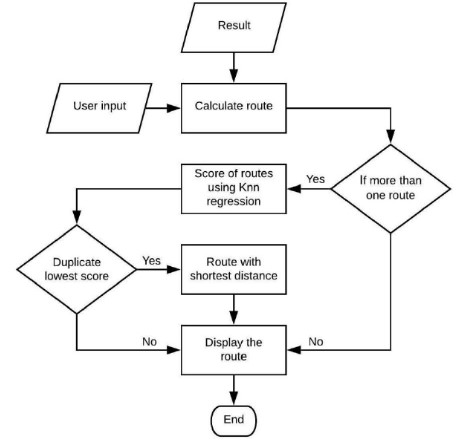
\includegraphics[width=0.35\textwidth]{2/figures/CondicionSafe.jpg}
		\caption{Flujo de condición para detectar rutas seguras}
		\label{1:fig2}
	\end{center}
\end{figure}
%\medskip

\subsubsection{Resultados obtenidos}
Se establece un punto de origen A y un punto de destino B en el distrito de Manhattan, dando como resultado que bajo el modelo de KNN Regressor, el R cuadrado de la puntuación de accidentes sea de 0.91 y la puntuación de criminalidad sea de 0.974; concluyendo que el modelo se ajusta mejor a sus datos.

%\medskip
\begin{figure}[h]
	\begin{center}
		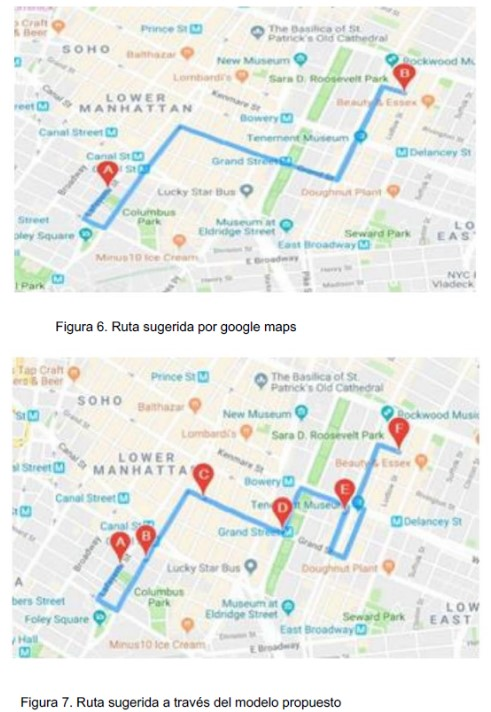
\includegraphics[width=0.4\textwidth]{2/figures/resultRoute.jpg}
		\caption{Resultados obtenidos}
		\label{1:fig2}
	\end{center}
\end{figure}
%\medskip

%%%%%%%%%%%%%%%%%%%%%%%%%%%%%%%%%%%%%%%%%%%%%%%%%%%%%%%%%%%%%%
%\medskip
\subsection{Real-time safest route identification: Examining the trade-off between safest and fastest routes \citep*{pr_Ghoul}}
\citeauthor{pr_Ghoul} realizaron un artículo de investigación el cual fue publicado en la revista «Analytic methods in accident research» en el año 2023. Este fue titulado \citetitle{pr_Ghoul} la cual traducida al español significa «Identificación de la ruta más segura en tiempo real: examen de la relación entre las rutas más seguras y las más rápidas»..

\subsubsection{Planteamiento del Problema y objetivo }
Este trabajo de investigación propone un nuevo enfoque de predicción de rutas seguras debido a la creciente congestión vehícular y accidentes, esto con el fin de mejorar el flujo vehícular  de un determinado sector utilizando datos en tiempo real para que se sincronice con el modelo y proporcionar avisos para que el usuario evite regiones congestionadas o que están expuestos a peligros en las carreteras. Tiene como objetivo desarrollar un algoritmo de enrutamiento en tiempo real bajo una métrica propuesta que combina el riesgo de accidentes con el tiempo de viaje a lo largo de diferentes puntos de una ruta.

\subsubsection{Metodología empleada por los autores}
Se utiliza un conjunto de datos de código abierto llamado pNEUMA, de la ciudad de Atenas, Grecia. Este conjunto de datos utiliza drones para recopilar los datos sobre el tráfico en horas pico, asimismo, bajo esta recopilación, se extrae los datos de la posición, velocidad, aceleración y tipo de vehículo. Luego se pre procesaron los datos mediante la comparación por pares de trayectorias. Después se calculó el tiempo de coalición (TTC) de cada ubicación para aplicarlo al modelo propuesto.
%\medskip
\begin{figure}[h]
	\begin{center}
		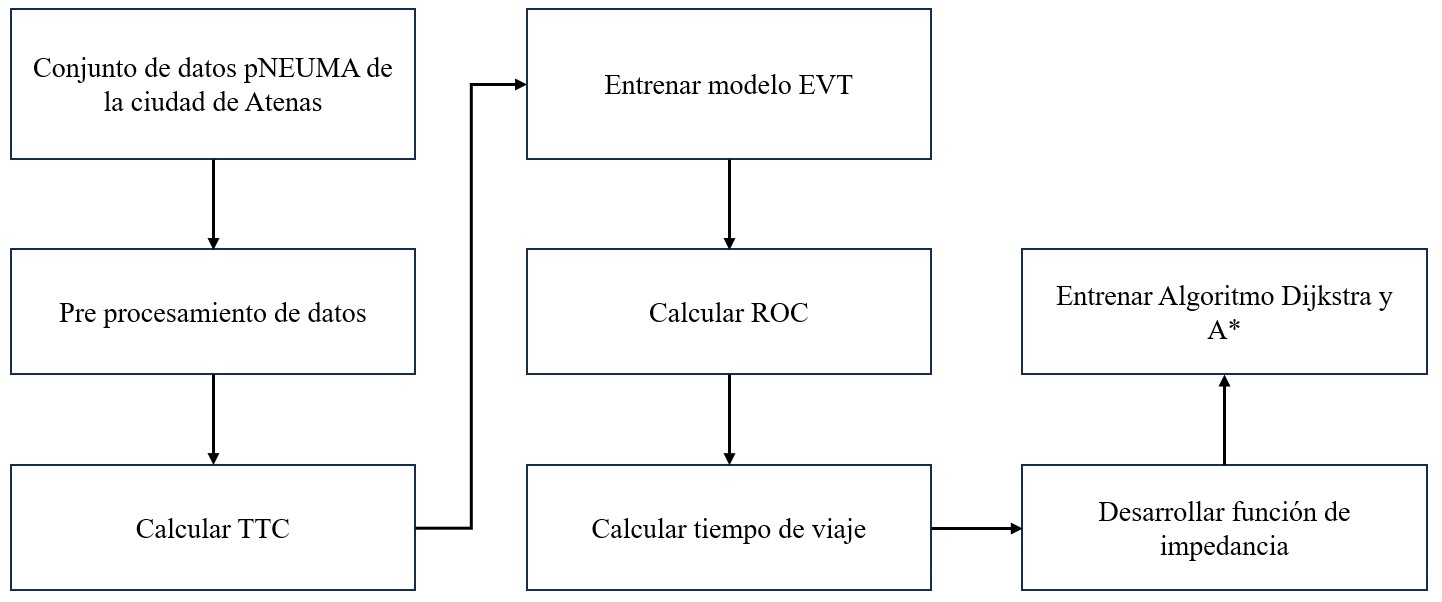
\includegraphics[width=0.65\textwidth]{2/figures/AtenaMetodo.jpg}
		\caption{Metodología propuesta por los autores}
		\label{1:fig2}
	\end{center}
\end{figure}
%\medskip

El modelo propuesto es un modelo de teoría de valores extremos (EVT), específicamente el modelo bayesiano jerárquico para estimar el riesgo de accidente de cada ubicación en tiempo real y se incorporan covariables para optimizar el rendimiento del modelo propuesto. Después de desarrollar el modelo bayesiano, se calcula el riesgo de colisión (ROC), que estima el número total de accidentes que se observan en una ubicación, también se calcula una métrica de tiempo de viaje para desarrollar una función de impedancia para realizar comparaciones entre los distintos nodos de una red de carreteras bajo un algoritmo de enrutamiento. Para el cálculo de la función de impedancia (S) es de la siguiente manera:

%\medskip
\begin{figure}[h]
	\begin{center}
		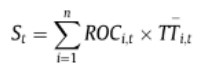
\includegraphics[width=0.35\textwidth]{2/figures/roc.jpg}
	\end{center}
\end{figure}
%\medskip

Posterior al cálculo de la función de impedancia, se utiliza en el algoritmo Dijkstra o el algoritmo A*. Después se desarrolla un algoritmo que elige la mejor ruta, el cuál identifica distintas rutas según la preferencia del usuario, tomando en cuenta tanto la seguridad como la movilidad.

\subsubsection{Resultados obtenidos}
Bajo la metodología propuesta, se encontró que el 23\% de las rutas más rápidas eran similares a las rutas más seguras. Además, la ruta más segura comparte en un 54\% los mismos enlaces que la ruta más rápida, existiendo un equilibrio entre seguridad y movilidad en distintos escenarios. Este trabajo de investigación aporta con un modelo de recomendación de rutas que presenta una buena eficacia en cuanto a cambios dinámicos en tiempo real en diferentes tipos de condiciones; sin embargo, para el cálculo de riesgo, depende de una percepción de seguridad más que la seguridad real, por lo que se recomienda que se establezca bajo su propia preferencia y prioridades, ya que es difícil cuantificar el riesgo real de un sector.

\subsection{A reinforcement learning-based routing algorithm for large street networks. \citep*{pr_diya}}
\citeauthor{pr_diya} realizaron un artículo de investigación el cual fue publicado en la « International Journal of Geographical Information Science» en el año 2024. Este fue titulado \citetitle{pr_diya} la cual traducida al español significa «Un algoritmo de enrutamiento basado en aprendizaje de refuerzo para grandes redes de calles».

\subsubsection{Planteamiento del Problema y objetivo }
Ante la problemática de contar con sistemas de evacuación y rutas de emergencia para minimizar los daños ocasionados durante los desastres naturales, los algoritmos tradicionales de enrutamiento cuentan con problemas de escalavidiad cuándo estas se enfrentan a evacuaciones a gran escala que involucran a diferentes rutas, asimismo, la complejidad computacional de estos algoritmos puede aumentar a medida que crece y se vuelve más complejo un escenario de evacuación, llevando a tener largos tiempos de cáculos, además que trabajan con pocos parámetros que capturan la complejidad y dinamismo de las emergencias por inundaciones. Ante estas limitaciones y con las contribuciones recientes de algoritmos de aprendizaje por refuerzo profundo (DRL), se desarrolló un algoritmo de aprendizaje por refuerzo para mejorar la eficiencia de enrutamiento en una gran red de carrenteras en tiempo real, para lograr dicho objetivo, se entrenó dicho algoritmo en una supercomputadora FASTER, que maneja grandes redes de carreteras de una base de datos espacial.

\subsubsection{Metodología empleada por los autores}
Se recopilan los datos de redes de transporte de la ciudad de Nueva York y Houston, que contienen la longitud y latitud de cada punto de interés, asimismo para los datos de transporte se exporta información cartográfica del área centra de Houston y la ciudad de Nueva York. 

Para el algoritmo de aprendizaje por refuerzo, el sistema de enrutamiento puede modelarse como una tupla de proceso de decisión de Markov (MDP. Cada tupla contiene el conjunto de estados de cada vértice, conjunto de acciones que considera la red neuronal durante el entrenamiento, la función de recompensa para optimizar la preferencia del usuario, donde se incorpora el factor de seguridad. Además, se establece políticas con el método de gradientes de políticas, el cual se conecta con el algoritmo de ascenso de gradiente estocástico. Para disminuir la varianza del estimado de gradientes del algorimo, se utiliza la Optimización de Política Proximal (PPO). 

%\medskip
\begin{figure}[h]
	\begin{center}
		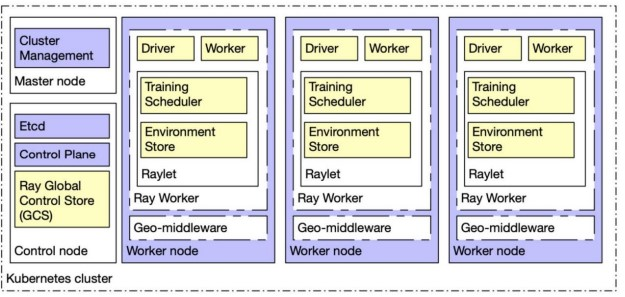
\includegraphics[width=0.65\textwidth]{2/figures/algoMod.jpg}
		\caption{Puntuaciones de evaluación}
		\label{1:fig2}
	\end{center}
\end{figure}
%\medskip

Para hacer frente a los entornos complejos y dinámicos, se requiere de una red neuronal que memorice los nodos y elija una acción válida a través de Q-learning, este algoritmo evita no seleccionar rutas inválidas con la red de políticas.

%\medskip
\begin{figure}[h]
	\begin{center}
		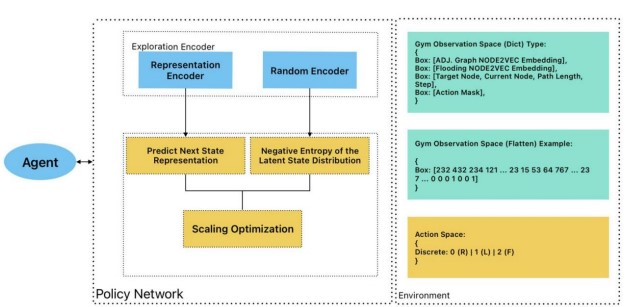
\includegraphics[width=0.65\textwidth]{2/figures/politica.jpg}
		\caption{Puntuaciones de evaluación}
		\label{1:fig2}
	\end{center}
\end{figure}
%\medskip

\subsubsection{Resultados obtenidos}
Se comparó con el método de Dijkstra y el algoritmo clásico de aprendiza por refuerzo mediante puntuación por métricas de seguridad y recompensa de cada ciudad, como también su tiempo. Los resultados indican que el mejor algoritmo es el modelo propuesto, ya que tienen un mayor puntaje de seguridad, como también un mayor indicador de recompensa. Sin embargo, tiene una mayor duración al ejecutar cada enrutamiento o detectar rutas seguras. También se destaca el hecho de que el modelo propuesto no atraviesa los puntos inundados, superando en términos de seguridad a los algoritmos tradicionales.

%\medskip
\begin{figure}[h]
	\begin{center}
		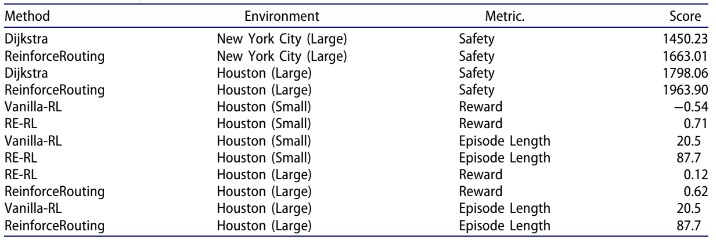
\includegraphics[width=0.65\textwidth]{2/figures/resultN.jpg}
		\caption{Puntuaciones de evaluación}
		\label{1:fig2}
	\end{center}
\end{figure}
%\medskip
